\documentclass[conference]{IEEEtran}
\IEEEoverridecommandlockouts
\usepackage{cite}
\usepackage{hyperref}
\usepackage{amsmath,amssymb,amsfonts}
\usepackage{algorithmic}
\usepackage{graphicx}
\usepackage{textcomp}
\usepackage{xcolor}
\usepackage{booktabs}
\usepackage{array}
\usepackage{tabularx}
\usepackage{tikz}
\usetikzlibrary{shapes.geometric, arrows.meta, positioning, fit, backgrounds}

\def\BibTeX{{\rm B\kern-.05em{\sc i\kern-.025em b}\kern-.08em
    T\kern-.1667em\lower.7ex\hbox{E}\kern-.125emX}}

\begin{document}

\begin{titlepage}
    \thispagestyle{empty}
    \centering
    \vspace*{0cm}

\begin{figure}[htbp]
    \centering
    \includegraphics[width=0.4\linewidth]{./figs/just_logo.JPG}
    \label{fig:logo}
\end{figure}

    {\large \textbf{GRADUATION PROJECT PROPOSAL -- GP1}}\\[1.0cm]

    {\Huge \textbf{A Closed-Loop Physiologically Adaptive Virtual Reality System for Exposure Therapy of Specific Phobias}}\\[1.5cm]

    {\large Final Project Proposal Submitted to \\
The Department of Computer Science \\
Faculty of Computer and Information Technology \\
Jordan University of Science and Technology \\
In Partial Fulfillment of the Requirements for the Degree of \\
Bachelor of Science in Computer Science}\\

    \vspace*{1cm}

    {\large \textbf{Prepared by:}}\\[0.4cm]
    {\large Hamzeh Badaro \texttt{[163343]}\\}
    {\large Eman Abu Zeitoun \texttt{[166016]}\\}
    {\large Husam Al-Zu'bi \texttt{[158032]}\\}
    {\large Dareen Halaweh \texttt{[161118]}\\}

    \vspace*{1cm}

    {\large \textbf{Supervised by:}\\}
    {\large Dr.\ Qanita Bani Baker}\\[1cm]

    \vfill

    {\large June 2026}

\end{titlepage}

\newpage
\begin{figure}[htbp]
    \centering
    \includegraphics[width=1\textwidth]{./figs/arabic_tanazol.JPG}
    \label{fig:tanazol}
\end{figure}


\title{A Closed-Loop Physiologically Adaptive Virtual Reality System for Exposure Therapy of Specific Phobias%
\thanks{Graduation Project Proposal -- GP1, Faculty of Computer \& Information Technology, Jordan University of Science and Technology.}%
}

\author{
\IEEEauthorblockN{Hamzeh Badaro}
\IEEEauthorblockA{\textit{Dept.\ Computer Science} \\
\textit{Jordan University of Science and Technology}\\
Irbid, Jordan \\
\texttt{hkbadaro22@cit.just.edu.jo}}
\and
\IEEEauthorblockN{Eman Abu Zeitoun}
\IEEEauthorblockA{\textit{Dept.\ Computer Science} \\
\textit{Jordan University of Science and Technology}\\
Irbid, Jordan \\
\texttt{eqabuzeitoun22@cit.just.edu.jo}}
\and
\IEEEauthorblockN{Husam Al-Zu'bi}
\IEEEauthorblockA{\textit{Dept.\ Computer Science} \\
\textit{Jordan University of Science and Technology}\\
Irbid, Jordan \\
\texttt{haalzubi21@cit.just.edu.jo}}
\and
\IEEEauthorblockN{Dareen Halaweh}
\IEEEauthorblockA{\textit{Dept.\ Computer Science} \\
\textit{Jordan University of Science and Technology}\\
Irbid, Jordan \\
\texttt{dhhalawa22@cit.just.edu.jo}}
}

\maketitle

\begin{abstract}
Mental health disorders affect approximately one in eight individuals globally, and treatment access in low- and middle-income countries remains severely limited. Specific phobias carry a lifetime prevalence of 7--12\% and impose significant clinical and socioeconomic burdens. Current virtual reality exposure therapy systems deliver stimuli at fixed intensities with no real-time physiological feedback, leaving a critical gap in adaptive therapeutic control.

This proposal describes CL-PAVE, a closed-loop physiologically adaptive virtual reality system. It reads continuous electrocardiogram data from a Polar H10 chest-strap sensor, extracts heart rate variability features in a Python inference layer, and sends a continuous arousal regression score to a standalone Meta Quest 3S running an Unreal Engine 5 therapeutic environment.

The system modulates in-scene stimulus parameters in real time, including ambient audio intensity, animation speed, and stimulus density, to keep physiological arousal within the therapeutic window defined by the inhibitory learning model of exposure therapy. Two phobia scenarios will validate the generalizability of the architecture.

The expected outcome is a working proof-of-concept showing that a fully mobile closed-loop biofeedback system can regulate therapeutic arousal with sub-second latency, filling a clear gap in current virtual reality therapy and laying groundwork for expansion to additional phobia subtypes.
\end{abstract}

\begin{IEEEkeywords}
Virtual Reality Exposure Therapy, Closed-Loop Biofeedback, Heart Rate Variability, Specific Phobias, Affective Computing, Unreal Engine 5.
\end{IEEEkeywords}

\section{PROJECT GOALS AND OBJECTIVES}

The primary objective is to design, implement, and validate a proof-of-concept (PoC) closed-loop physiologically adaptive VR system, CL-PAVE, for specific phobias. The system uses real-time electrocardiogram (ECG) analysis to keep therapeutic arousal at the right level through continuous scene modulation on a standalone head-mounted display (HMD).

The specific aims are as follows:

\begin{enumerate}
    \item \textbf{Aim 1 (System Integration):} Establish an end-to-end pipeline connecting the Polar H10 via Bluetooth Low Energy (BLE) to a Python inference layer, bridging the output to a Meta Quest 3S Unreal Engine 5 (UE5) application via Open Sound Control (OSC) protocol, with a target latency of $<$1.0 second.

    \item \textbf{Aim 2 (Arousal Estimation Engine):} Develop a continuous arousal regression model based on Heart Rate Variability (HRV) metrics (HR, RMSSD, SDNN), calibrated against individualized baselines and validated via Subjective Units of Distress Scale (SUDS) feedback.

    \item \textbf{Aim 3 (Modulation Mechanics):} Implement continuous, bidirectional modulation of environmental variables (sound intensity, animation speed, stimulus density) to regulate user arousal without breaking immersion via discrete scene transitions. Stimulus intensity decreases as arousal exceeds therapeutic thresholds and increases as arousal falls below them.

    \item \textbf{Aim 4 (Generalizability Assessment):} Validate the generic architecture by demonstrating functionality across at least two distinct phobia scenarios (acrophobia and arachnophobia) using a unified logic framework.

    \item \textbf{Aim 5 (Data Infrastructure):} Develop automated logging capabilities for subsequent clinical analysis and algorithm refinement.
\end{enumerate}

\section{INTRODUCTION}

\subsection{Background}

Mental health disorders affect approximately one in eight individuals globally, yet in low- and middle-income countries fewer than 30\% of those affected receive adequate treatment \cite{roccaforte2026}. Specific phobias represent a significant portion of this clinical burden. The Diagnostic and Statistical Manual of Mental Disorders, 5th edition, Text Revision (DSM-5-TR) categorizes them as an intense, persistent fear of a stimulus that is disproportionate to the actual danger it poses \cite{dsm5tr2022}, with lifetime prevalence estimated between 7\% and 12\% \cite{krijn2004}.

Without treatment, specific phobias can lead to workplace absenteeism, reduced quality of life, and increased strain on mental health infrastructure \cite{khanna2022}. Exposure therapy remains the most empirically supported treatment, particularly Graded Exposure Therapy (GET), which is predicated on the inhibitory learning model \cite{craske2014}. This approach does not erase the fear response; rather, repeated exposure facilitates the formation of new inhibitory memories that compete with the original fear memory during retrieval \cite{craske2014}.

For this mechanism to work, exposure intensity has to stay within a specific therapeutic window. It must be high enough to activate the fear network, yet kept under control so the patient does not disengage or drop out. Holding the intensity in that window has traditionally depended on the therapist reading the patient in real time, usually without any objective physiological markers to rely on.

Virtual Reality Exposure Therapy (VRET) has demonstrated efficacy comparable to in-vivo exposure across multiple phobia subtypes. Rothbaum et al.\ established early evidence for aviophobia \cite{rothbaum2000}, Garcia-Palacios et al.\ demonstrated controlled efficacy for arachnophobia \cite{garcia2002}, and a protocol comparing CBT-enhanced adaptive VRET against in-vivo treatment for social anxiety \cite{cbtvr2022} added further support for the approach. A significant randomized controlled trial (RCT) by Miloff et al.\ demonstrated that a single gamified VR session on consumer-grade hardware was non-inferior to traditional therapy for spider phobia, with 95\% of participants maintaining clinical gains after one year \cite{miloff2024}. While this evidence supports the clinical readiness of consumer VR hardware, current commercial systems (e.g., Limbix, Psious) primarily offer static or semi-static environments without real-time physiological integration \cite{ferreira2025}.

HRV, derived from ECG data, is a well-established biomarker for Autonomic Nervous System (ANS) activity during anxiety and fear \cite{tsai2025,nummenmaa2014}. Ritsert et al.\ confirmed that heart and breathing rate variations reliably distinguish anxiety states across controlled experimental conditions \cite{ritsert2022}, and Battaglia et al.\ demonstrated instantaneous spectral HRV changes during human fear learning, directly linking HRV dynamics to the fear acquisition process \cite{battaglia2020}. Interactive VR systems that deliver real-time HRV biofeedback have demonstrated measurable reductions in self-reported anxiety \cite{xu2025}. Modern hardware, such as the Polar H10 chest-belt sensor, provides clinically validated ECG data with near-perfect agreement to medical-grade Lead II ECG \cite{chung2026}, making it a viable choice for unobtrusive clinical deployment \cite{skala2022}. Specific HRV features such as RMSSD, the LF/HF ratio, and SDNN have been validated as effective inputs for machine learning models that classify stress and fear \cite{tsai2025,sajno2023,esc1996}. Kumar and Haider applied these same biosignal features to emotion recognition for stress and anxiety detection \cite{kumar2025}, while He et al.\ reviewed and compared a range of such models and found they generalize reasonably well across anxiety detection contexts \cite{he2025}. A systematic review by Ancillon et al.\ reached a similar conclusion across several sensor modalities \cite{ancillon2022}.

\subsection{Problem Statement and Knowledge Gap}

Both VRET and real-time physiological sensing are mature, yet a standalone fully integrated closed-loop system has not been widely deployed. Four gaps stand out in the literature:

\textbf{Gap 1 (Lack of Continuous Within-Session Adaptation):} While ``semi-adaptive'' systems exist that adjust difficulty between sessions based on retrospective review \cite{leong2025}, current market solutions do not offer continuous, intra-session modulation of scene elements driven by real-time ECG data \cite{leong2025,orozco2024}.

\textbf{Gap 2 (Absence of Standalone Mobile Closed-Loop Systems):} Published closed-loop or adaptive VR therapy systems currently depend on tethered PCs or dedicated laboratory infrastructure \cite{orozco2024,mevlevio2024,vet2025}. Moon et al.\ specifically noted that cybersickness and presence effects in VR-biofeedback systems for depression and anxiety were evaluated only under fixed laboratory conditions, with no pathway toward standalone mobile deployment \cite{moon2025}. Although modern mobile hardware (e.g., Meta Quest 3S) possesses the computational capability for concurrent rendering and bio-signal inference, a fully validated mobile system remains undocumented.

\textbf{Gap 3 (Immersion Disruption via Explicit Feedback):} Displaying direct physiological metrics (e.g., numerical heart rate) during a session can compromise therapeutic presence \cite{leong2025}. Sahebi \cite{sahebi2024} demonstrated that intrusive HCI feedback during real-time panic monitoring disrupts the user experience, while Chiossi et al.\ showed that optimizing visual complexity for physiologically-adaptive VR systems requires indirect, environmental cues rather than explicit overlays \cite{chiossi2024}. Adjusting ambient audio and animation speed as indirect feedback has not been explored enough as a non-intrusive alternative.

\textbf{Gap 4 (Single-Phobia Limitations):} Existing adaptive VR systems are typically engineered for a single specific phobia \cite{vet2025,mevlevio2024}, necessitating custom development for each new clinical application. A generalized architecture capable of accommodating various phobias simply by replacing visual assets is currently lacking.

\subsection{Hypothesis}

A real-time closed-loop system using a Polar H10 for continuous ECG acquisition, processed via a Python-based ML engine, can modulate VR scene parameters on a Meta Quest 3S in real time. The hypothesis is that this keeps patient arousal inside the therapeutic window during graded exposure therapy for specific phobias, reducing reliance on manual therapist adjustment.

\subsection{Significance of Work}

CL-PAVE brings together clinical psychology, affective computing, and immersive technology. The idea of biofeedback-driven adaptive virtual spaces, in which physiological signals continuously reshape the digital environment, has been proposed as a foundation for human-computer interaction \cite{ghandi2019}. Closing the loop between physiology and the VR environment could improve treatment outcomes while easing the load on the therapist. And because the system runs on affordable consumer hardware, the same core could later be carried over to other anxiety disorders without rebuilding it from scratch.

\section{REVIEW AND ANALYSIS OF RELATED WORK}

The work draws on five areas: closed-loop bioengineering frameworks, VRET clinical efficacy, biosignal processing for anxiety classification, hardware validation, and adaptive VR design. Table~\ref{tab:related_work} summarizes the foundational literature.

\begin{table}[h!]
\centering
\caption{Summary of Related Works}
\label{tab:related_work}
\resizebox{\columnwidth}{!}{%
\begin{tabular}{|p{0.07\columnwidth}|p{0.22\columnwidth}|p{0.33\columnwidth}|p{0.33\columnwidth}|}
\hline
\textbf{Ref.} & \textbf{Authors \& Year} & \textbf{Title / Contribution} & \textbf{Relevance to This Work} \\ \hline
\cite{roccaforte2026} & Roccaforte et al., 2026 & Towards a Closed-Loop Bioengineering Framework & Defines closed-loop bioengineering; roadmap for sensor scaling. \\ \hline
\cite{ferreira2025} & Ferreira et al., 2025 & Biofeedback Systems for Psychological Well-Being & Validates VR delivery; proves adherence and self-regulation improvements. \\ \hline
\cite{leong2025} & Leong, 2025 & VR in Phobia Treatment and Emotional Resilience & Reveals gap between semi-adaptive vs.\ continuous loop systems. \\ \hline
\cite{orozco2024} & Orozco-Mora et al., 2024 & Dynamic Difficulty Adaptation Based on Stress Detection & Technical precedent for adaptive VR loops; validates control laws. \\ \hline
\cite{mevlevio2024} & Mevlevi\v{o}\v{g}lu \& Tabirca, 2024 & CNN for Real-Time Anxiety Classification in VR Therapy & Blueprint for 10-second windowing and 3-class anxiety output. \\ \hline
\cite{chung2026} & Chung et al., 2026 & Validity of the Polar H10 for HR and Synchrony & Confirms Polar H10 achieves near-perfect agreement with clinical ECG. \\ \hline
\cite{miloff2024} & Miloff et al., 2024 & Single-Session VR Exposure Therapy vs.\ Traditional & RCT evidence validating consumer VR efficacy for specific phobias. \\ \hline
\cite{vet2025} & Healthcare (VET), 2025 & Predictive and Adaptive VR Exposure for Spider Fear & Closest published system; limited to a single phobia type. \\ \hline
\cite{ghandi2019} & Ghandi, 2019 & Cyber-Physical Emotive Spaces: Biofeedback Interaction & Foundational theory of biofeedback-driven adaptive virtual spaces. \\ \hline
\cite{craske2014} & Craske et al., 2014 & Maximizing Exposure Therapy: Inhibitory Learning & Clinical foundation defining the mechanism of exposure therapy efficacy. \\ \hline
\end{tabular}%
}
\end{table}

Four existing systems serve as primary benchmarks:

\textbf{PhoVR} \cite{orozco2024} uses HR and Electrodermal Activity (EDA) to modulate scene elements. However, it relies on tethered PC hardware and Galvanic Skin Response (GSR) sensors, which present latency and artifact challenges in VR environments.

\textbf{Virtual Exposure Therapist (VET)} \cite{vet2025} is a recent multimodal predictive system for arachnophobia. It remains a research prototype focused on a single phobia, without clear adaptation for standalone mobile development.

\textbf{Leong (2025) Semi-Adaptive VRET} \cite{leong2025} proposes multi-phobia scalability but relies on inter-session adaptation based on retrospective therapist review, rather than real-time physiological data.

\textbf{Mevlevi\v{o}\v{g}lu \& Tabirca (2024)} \cite{mevlevio2024} provides a validated classification architecture using 10-second ECG windows, but lacks a downstream VR environmental modulation layer to act upon the classification.

\section{APPROACH AND METHODOLOGY}

\subsection{System Architecture Overview}

The CL-PAVE system operates on a continuous four-stage cycle, illustrated in Fig.~\ref{fig:architecture}:

\begin{enumerate}
    \item \textbf{ECG Acquisition:} The Polar H10 transmits R-R interval data via BLE at 130\,Hz to an edge processing device.
    \item \textbf{Data Processing \& Inference:} A Python script extracts HRV features (HR, RMSSD, SDNN) over 10-second sliding windows. A regression model, calibrated against a pre-session individualized baseline, outputs a continuous arousal score to drive environmental adaptation.
    \item \textbf{Environmental Adaptation:} The arousal score is transmitted via OSC to the UE5 application on the Meta Quest 3S. Scene parameters are continuously adjusted using linear interpolation over 2--3 seconds. Stimulus intensity decreases when arousal exceeds the therapeutic window and increases when arousal falls below it.
    \item \textbf{Feedback \& Recalibration:} The system continuously logs data and recalculates metrics to form a closed responsive loop.
\end{enumerate}

\begin{figure}[h!]
\centering
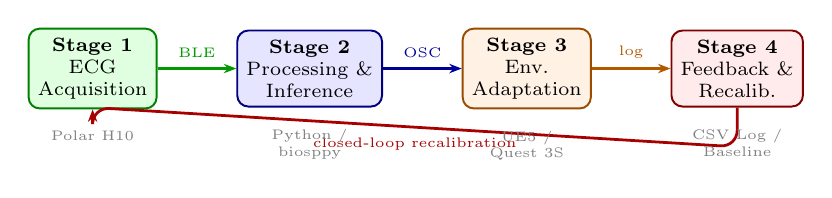
\begin{tikzpicture}[
    font=\scriptsize,
    node distance=0.45cm,
    stage/.style={rectangle, rounded corners=4pt, draw, align=center,
                  minimum width=1.6cm, minimum height=0.75cm,
                  line width=0.7pt},
    arr/.style={-{Stealth[length=4.5pt]}, line width=1pt},
]
\node[stage, fill=green!12, draw=green!50!black]
    (s1) {\textbf{Stage 1}\\ECG\\Acquisition};
\node[stage, fill=blue!10, draw=blue!50!black, right=1.0cm of s1]
    (s2) {\textbf{Stage 2}\\Processing \&\\Inference};
\node[stage, fill=orange!10, draw=orange!60!black, right=1.0cm of s2]
    (s3) {\textbf{Stage 3}\\Env.\\ Adaptation};
\node[stage, fill=red!8, draw=red!50!black, right=1.0cm of s3]
    (s4) {\textbf{Stage 4}\\Feedback \&\\Recalib.};

\draw[arr, green!60!black]   (s1.east) -- node[above,font=\tiny]{BLE} (s2.west);
\draw[arr, blue!60!black]    (s2.east) -- node[above,font=\tiny]{OSC} (s3.west);
\draw[arr, orange!70!black]  (s3.east) -- node[above,font=\tiny]{log} (s4.west);

\draw[arr, red!65!black, rounded corners=6pt]
    (s4.south) -- ++(0,-0.5)
    -- node[below, font=\tiny, align=center]{\textcolor{red!65!black}{closed-loop recalibration}}
    (s1.south |- s4.south) -- (s1.south);

\node[font=\tiny, gray, below=0.15cm of s1, align=center] {Polar H10};
\node[font=\tiny, gray, below=0.15cm of s2, align=center] {Python /\\biosppy};
\node[font=\tiny, gray, below=0.15cm of s3, align=center] {UE5 /\\Quest 3S};
\node[font=\tiny, gray, below=0.15cm of s4, align=center] {CSV Log /\\Baseline};
\end{tikzpicture}
\caption{CL-PAVE four-stage closed-loop pipeline. Stage~1: the Polar H10 acquires raw ECG at 130\,Hz over BLE. Stage~2: the Python layer extracts HRV features (HR, RMSSD, SDNN) and outputs a continuous arousal score. Stage~3: the score is transmitted via OSC to the UE5 runtime on the Meta Quest 3S for real-time scene modulation. Stage~4: session data are logged and the baseline is recalibrated, closing the loop back to Stage~2.}
\label{fig:architecture}
\end{figure}

\subsection{Hardware and Software Stack}

\begin{itemize}
    \item \textbf{Biosensor:} Polar H10 chest-strap ECG (selected for superior artifact resilience and accuracy compared to optical or GSR sensors) \cite{chung2026,skala2022}.
    \item \textbf{HMD:} Meta Quest 3S (standalone, no tethered PC required).
    \item \textbf{Processing Layer:} Python 3.x using \texttt{biosppy} and \texttt{neurokit2} for real-time HRV feature extraction.
    \item \textbf{VR Engine:} Unreal Engine 5 with Meta XR SDK.
    \item \textbf{Communication Protocol:} Open Sound Control (OSC) via built-in UE5 plugin.
\end{itemize}

\subsection{Arousal Regression Model}

CL-PAVE uses a regression model rather than discrete class labels, outputting a continuous arousal score $a(t) \in [0, 1]$. Input features are computed over a 10-second sliding window:

\begin{equation}
a(t) = f\!\left(\mathrm{HR}(t),\, \mathrm{RMSSD}(t),\, \mathrm{SDNN}(t)\right)
\label{eq:arousal}
\end{equation}

where each feature is normalized against the patient's pre-session baseline. The therapeutic window is defined as $a(t) \in [\theta_{\mathrm{low}},\, \theta_{\mathrm{high}}]$, and the modulation signal $m(t)$ applied to scene parameters is computed as:

\begin{equation}
m(t) = \begin{cases}
-k\bigl(a(t) - \theta_{\mathrm{high}}\bigr) & \text{if } a(t) > \theta_{\mathrm{high}} \\
+k\bigl(\theta_{\mathrm{low}} - a(t)\bigr) & \text{if } a(t) < \theta_{\mathrm{low}} \\
0 & \text{otherwise}
\end{cases}
\label{eq:modulation}
\end{equation}

where $k$ is a gain constant calibrated per session. SUDS ratings collected at 5-minute intervals serve as ground-truth labels for model calibration and validation.

\subsection{VR Scene Design and Clinical Protocol}

The system features modular environments:

\begin{itemize}
    \item \textbf{Acrophobia Scenario:} Varying height levels with modulating wind audio and cloud animation speed.
    \item \textbf{Arachnophobia Scenario:} Modulating ambient audio and spider entity movement speed.
\end{itemize}

Scene modulation itself serves as the safety mechanism. As arousal approaches a critical threshold, the stimulus elements inside the active environment are gradually reduced, which removes the need for discrete scene switching and keeps therapeutic immersion intact \cite{chiossi2024,leong2025}.

\begin{figure}[h!]
\centering
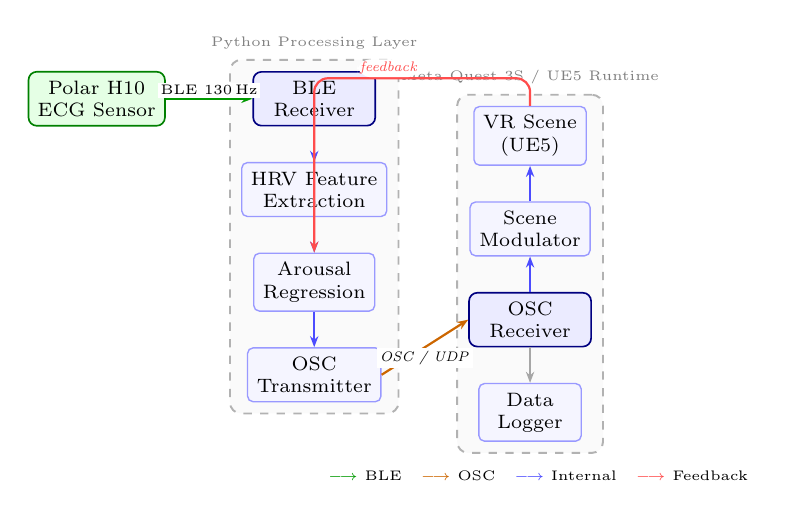
\begin{tikzpicture}[
    font=\scriptsize,
    node distance=0.55cm and 0.4cm,
    box/.style={rectangle, rounded corners=3pt, draw, align=center,
                minimum width=1.55cm, minimum height=0.65cm,
                fill=blue!8, draw=blue!50!black, line width=0.6pt},
    subbox/.style={rectangle, rounded corners=2pt, draw, align=center,
                   minimum width=1.3cm, minimum height=0.52cm,
                   fill=blue!4, draw=blue!40, line width=0.5pt},
    groupbox/.style={rectangle, rounded corners=4pt, draw=gray!60,
                     dashed, line width=0.7pt, fill=gray!4},
    arr/.style={-{Stealth[length=4pt]}, line width=0.8pt, draw=#1},
    lbl/.style={font=\tiny, fill=white, inner sep=1pt}
]
\node[box, fill=green!10, draw=green!50!black]
    (sensor) {Polar H10\\ECG Sensor};

\node[box, right=1.1cm of sensor]
    (ble)    {BLE\\Receiver};
\node[subbox, below=0.45cm of ble]
    (hrv)    {HRV Feature\\Extraction};
\node[subbox, below=0.45cm of hrv]
    (model)  {Arousal\\Regression};
\node[subbox, below=0.45cm of model]
    (osc)    {OSC\\Transmitter};

\begin{scope}[on background layer]
\node[groupbox, fit=(ble)(hrv)(model)(osc),
      inner sep=4pt, label={[font=\tiny,gray]above:Python Processing Layer}]
    (pygroup) {};
\end{scope}

\node[box, right=1.1cm of osc, yshift=0.7cm]
    (oscRx)  {OSC\\Receiver};
\node[subbox, above=0.45cm of oscRx]
    (mod)    {Scene\\Modulator};
\node[subbox, above=0.45cm of mod]
    (scene)  {VR Scene\\(UE5)};
\node[subbox, below=0.45cm of oscRx]
    (log)    {Data\\Logger};

\begin{scope}[on background layer]
\node[groupbox, fit=(scene)(mod)(oscRx)(log),
      inner sep=4pt,
      label={[font=\tiny,gray]above:Meta Quest 3S / UE5 Runtime}]
    (uegroup) {};
\end{scope}

\draw[arr=green!60!black]
    (sensor.east) -- node[lbl, above]{BLE 130\,Hz} (ble.west);
\draw[arr=blue!70] (ble.south)   -- (hrv.north);
\draw[arr=blue!70] (hrv.south)   -- (model.north);
\draw[arr=blue!70] (model.south) -- (osc.north);
\draw[arr=orange!80!black]
    (osc.east) -- node[lbl, below]{\textit{OSC / UDP}} (oscRx.west);
\draw[arr=blue!70] (oscRx.north) -- (mod.south);
\draw[arr=blue!70] (mod.north)   -- (scene.south);
\draw[arr=gray!70] (oscRx.south) -- (log.north);
\draw[arr=red!70, rounded corners=5pt]
    (scene.north) -- ++(0, 0.35)
    -| node[lbl, above left, pos=0.25]{\textcolor{red!70}{\textit{feedback}}} (model.north);

\node[font=\tiny, align=left, below=0.25cm of log, xshift=0.1cm]{%
    \textcolor{green!60!black}{$\longrightarrow$} BLE\quad
    \textcolor{orange!80!black}{$\longrightarrow$} OSC\quad
    \textcolor{blue!70}{$\longrightarrow$} Internal\quad
    \textcolor{red!70}{$\longrightarrow$} Feedback};
\end{tikzpicture}
\caption{Component interaction diagram of CL-PAVE. The Polar H10 streams raw ECG over BLE at 130\,Hz to the Python processing layer, which extracts HRV features and outputs a continuous arousal score transmitted via OSC/UDP to the UE5 runtime on the Meta Quest 3S. The UE5 modulator adjusts scene parameters in real time; a feedback path recalibrates the regression baseline continuously, closing the loop.}
\label{fig:components}
\end{figure}

The clinical protocol consists of:
\begin{enumerate}
    \item A 3-minute resting baseline calibration (ECG recording, individualized threshold computation).
    \item A brief psychoeducation onboarding phase (approximately 2 minutes).
    \item A 20--30-minute graded exposure session with continuous closed-loop modulation.
    \item A post-session clinical assessment (SUDS, session debrief).
\end{enumerate}

\subsection{Data Logging}

All session data are automatically logged to a timestamped CSV file with the following schema:

\begin{center}
\texttt{timestamp | HR | HRV | arousal\_score | event\_type | scene\_element | scene\_value}
\end{center}

This log supports retrospective clinical analysis, session replay, and model refinement across participants.

\subsection{LOCATION AND SAFETY CONSIDERATIONS}

All development and PoC validation activities will be conducted within the Faculty of Computer \& Information Technology at Jordan University of Science and Technology (JUST), Irbid, Jordan.

Participant safety is managed through in-scene stimulus modulation: as arousal approaches a critical threshold, scene intensity is automatically attenuated, serving as the primary safety mechanism without requiring discrete environment switching. Sessions will be supervised by a researcher present in the room. No patient data will be transmitted off-device during PoC testing; all logs remain local to the device.

\section{PRELIMINARY RESULTS AND CURRENT STATUS}

Work is in the late architecture and prototyping phase. Table~\ref{tab:status} summarizes component status.

\begin{table}[h!]
\centering
\caption{Current Development Status of CL-PAVE Components}
\label{tab:status}
\resizebox{\columnwidth}{!}{%
\begin{tabular}{|p{0.35\columnwidth}|p{0.15\columnwidth}|p{0.45\columnwidth}|}
\hline
\textbf{Component} & \textbf{Status} & \textbf{Notes} \\ \hline
System architecture design & \textcolor{green!60!black}{Complete} & Validated against clinical and technical literature. \\ \hline
Hardware procurement & \textcolor{green!60!black}{Complete} & Polar H10 and Meta Quest 3S sourced and confirmed available. \\ \hline
HRV feature extraction (Python) & In Progress & \texttt{biosppy}/\texttt{neurokit2} pipeline under development; BLE connection script drafted. \\ \hline
Arousal regression model & Pending & Feature extraction must be complete; SUDS labels collected during pilot sessions. \\ \hline
UE5 OSC receiver module & In Progress & UE5 project initialized; OSC plugin configured; scene blueprints in design. \\ \hline
Acrophobia VR scenario & In Progress & Height environment and wind audio modulation under construction. \\ \hline
Arachnophobia VR scenario & Pending & Asset selection complete; scene construction pending UE5 pipeline finalization. \\ \hline
End-to-end latency validation & Pending & Target: $<$1.0\,s round-trip. Requires integrated pipeline. \\ \hline
SUDS-calibrated model validation & Pending & Requires pilot session data. \\ \hline
\end{tabular}%
}
\end{table}

\subsection{EXPECTED RESULTS/OUTPUTS}

Deliverables at PoC completion:

\begin{itemize}
    \item A functional end-to-end closed-loop pipeline with a demonstrated latency of $<$1.0\,s.
    \item Two validated VR therapy scenarios (acrophobia and arachnophobia) demonstrating architecture generalizability.
    \item A trained and SUDS-calibrated arousal regression model.
    \item Session log datasets suitable for retrospective clinical analysis.
    \item A documented open-source codebase (GitHub repository) covering the Python inference layer and UE5 OSC integration.
\end{itemize}

\newpage
\bibliographystyle{ieeetr}
\bibliography{references}

\end{document}
